\documentclass[a4paper,12pt]{article}
\usepackage[czech]{babel}
\usepackage[utf8]{inputenc}
\usepackage[T1]{fontenc}
\usepackage{graphicx}
\usepackage{amsmath}
\usepackage{amssymb}
\usepackage{hyperref}
\usepackage{listings}
\usepackage{xcolor}
\usepackage{booktabs}
\usepackage{float}
\usepackage{tikz}
\usepackage{pgfplots}
\usepackage{caption}
\usepackage{subcaption}

% Nastavení cest k obrázkům
\graphicspath{{../grafy/}}

% Nastavení stylu kódu
\definecolor{codegreen}{rgb}{0,0.6,0}
\definecolor{codegray}{rgb}{0.5,0.5,0.5}
\definecolor{codepurple}{rgb}{0.58,0,0.82}
\definecolor{backcolour}{rgb}{0.95,0.95,0.92}

\lstdefinestyle{mystyle}{
    backgroundcolor=\color{backcolour},   
    commentstyle=\color{codegreen},
    keywordstyle=\color{magenta},
    numberstyle=\tiny\color{codegray},
    stringstyle=\color{codepurple},
    basicstyle=\ttfamily\small,
    breakatwhitespace=false,         
    breaklines=true,                 
    captionpos=b,                    
    keepspaces=true,                 
    numbers=left,                    
    numbersep=5pt,                  
    showspaces=false,                
    showstringspaces=false,
    showtabs=false,                  
    tabsize=2
}

\lstset{style=mystyle}

% Nastavení hypertextových odkazů
\hypersetup{
    colorlinks=true,
    linkcolor=blue,
    filecolor=magenta,      
    urlcolor=cyan,
    pdftitle={Zpráva o predikci klíčových bodů},
    pdfpagemode=FullScreen,
}

\title{Predikce klíčových bodů s využitím algoritmu Random Forest}
\author{Jméno Příjmení\\Umělá inteligence a strojové učení}
\date{\today}

\begin{document}

\begin{titlepage}
    \centering
    \vspace*{1cm}
    {\scshape\LARGE Vysoká škola báňská - Technická univerzita Ostrava \par}
    \vspace{1cm}
    {\scshape\Large Fakulta elektrotechniky a informatiky\par}
    \vspace{1.5cm}
    {\huge\bfseries Predikce klíčových bodů s využitím algoritmu Random Forest\par}
    \vspace{2cm}
    {\Large\itshape Jméno Příjmení\par}
    \vspace{1cm}
    {\large Umělá inteligence a strojové učení\par}
    \vfill
    
    % Zde můžete přidat logo univerzity, pokud máte
    % \includegraphics[width=0.4\textwidth]{logo_univerzity.png}\\
    % \vspace{1cm}
    
    {\large \today\par}
\end{titlepage}

\tableofcontents
\newpage

\section{Úvod}
\label{sec:introduction}

Tato zpráva popisuje metodu predikce klíčových bodů s využitím algoritmu Random Forest. Predikce klíčových bodů je důležitou součástí mnoha aplikací počítačového vidění, od sledování pohybu objektů až po detekci a rozpoznávání obličejů. V této práci jsme se zaměřili na zpřesnění predikce pomocí pokročilých technik strojového učení.

Klíčovým cílem našeho přístupu bylo porovnání dvou metod:
\begin{itemize}
    \item \textbf{Bod s největší vahou} - základní metoda, která vybírá predikci s nejvyšší váhou
    \item \textbf{Random Forest} - pokročilá metoda využívající ensemble learning pro zlepšení predikce
\end{itemize}

Naše implementace je zaměřena na zpracování datové sady obsahující informace o klíčových bodech, jejich predikovaných pozicích a váhách. Vytvořili jsme robustní systém, který dokáže:

\begin{enumerate}
    \item Zpracovat vstupní data a identifikovat klíčové body
    \item Vytvořit příznakové vektory pro predikci
    \item Natrénovat modely Random Forest pro každý klíčový bod
    \item Porovnat výsledky s jednodušší metodou výběru bodu s největší vahou
    \item Vizualizovat a analyzovat výsledky
\end{enumerate}

\section{Teoretický základ}
\label{sec:theory}

\subsection{Klíčové body a jejich význam}
Klíčové body (keypoints) jsou specifické body v obraze, které jsou robustní vůči změnám osvětlení, rotaci, měřítku a dalším transformacím. V našem kontextu se jedná o body, které mohou představovat významné části objektů nebo anatomické body na lidském těle.

\subsection{Random Forest}
Random Forest je ensemble learning metoda pro klasifikaci, regresi a další úlohy. Funguje na principu vytvoření mnoha rozhodovacích stromů v průběhu trénování. Výstupem v případě regresní úlohy je průměr predikcí jednotlivých stromů. Hlavní výhody:

\begin{itemize}
    \item Odolnost vůči přeučení
    \item Schopnost zpracovat velké množství příznaků
    \item Přirozená schopnost určit důležitost jednotlivých příznaků
    \item Robustnost vůči šumu a outlierům
\end{itemize}

Matematicky můžeme Random Forest regresor definovat jako:

\begin{equation}
\hat{f}(x) = \frac{1}{B}\sum_{b=1}^{B}T_b(x)
\end{equation}

kde $\hat{f}(x)$ je predikce modelu, $B$ je počet stromů a $T_b(x)$ je predikce $b$-tého stromu pro vstup $x$.

\subsection{Vyhodnocení přesnosti}
Pro vyhodnocení přesnosti predikcí jsme použili střední kvadratickou chybu (Mean Squared Error - MSE):

\begin{equation}
MSE = \frac{1}{n}\sum_{i=1}^{n}(y_i - \hat{y}_i)^2
\end{equation}

kde $y_i$ jsou skutečné hodnoty a $\hat{y}_i$ jsou predikované hodnoty.

\section{Návrh řešení}
\label{sec:design}

\subsection{Struktura datového toku}

Pro lepší pochopení našeho přístupu je níže zobrazen diagram datového toku v našem systému:

\begin{figure}[H]
\centering
\begin{tikzpicture}[node distance=2cm and 2cm]
    % Definice uzlů
    \node (data) [draw, rounded corners, minimum width=3cm, minimum height=1cm] {Načtení dat};
    \node (keypoints) [draw, rounded corners, minimum width=3cm, minimum height=1cm, below=of data] {Identifikace klíčových bodů};
    \node (split) [draw, rounded corners, minimum width=3cm, minimum height=1cm, below=of keypoints] {Rozdělení dat};
    \node (features) [draw, rounded corners, minimum width=3cm, minimum height=1cm, below=of split] {Vytvoření příznaků};
    
    \node (baseline) [draw, rounded corners, minimum width=3cm, minimum height=1cm, left=of features] {Výpočet baseline};
    \node (training) [draw, rounded corners, minimum width=3cm, minimum height=1cm, below=of features] {Trénování modelu};
    \node (prediction) [draw, rounded corners, minimum width=3cm, minimum height=1cm, below=of training] {Predikce};
    \node (evaluation) [draw, rounded corners, minimum width=3cm, minimum height=1cm, below=of prediction] {Vyhodnocení};
    \node (visualization) [draw, rounded corners, minimum width=3cm, minimum height=1cm, below=of evaluation] {Vizualizace};
    \node (export) [draw, rounded corners, minimum width=3cm, minimum height=1cm, below=of visualization] {Export výsledků};
    
    % Propojení uzlů
    \draw[->] (data) -- (keypoints);
    \draw[->] (keypoints) -- (split);
    \draw[->] (split) -- (features);
    \draw[->] (features) -- (training);
    \draw[->] (split) -- (baseline);
    \draw[->] (training) -- (prediction);
    \draw[->] (baseline) -| (evaluation);
    \draw[->] (prediction) -- (evaluation);
    \draw[->] (evaluation) -- (visualization);
    \draw[->] (visualization) -- (export);
\end{tikzpicture}
\caption{Diagram datového toku systému predikce klíčových bodů}
\label{fig:dataflow}
\end{figure}

\subsection{Architektura systému}

Celý systém je rozdělen do následujících modulů:

\begin{figure}[H]
\centering
\begin{tikzpicture}[node distance=1.5cm]
    % Definice stylů
    \tikzstyle{module} = [draw, rounded corners, fill=blue!10, minimum width=3cm, minimum height=1cm]
    \tikzstyle{data} = [draw, rounded corners, fill=green!10, minimum width=3cm, minimum height=1cm]
    \tikzstyle{process} = [draw, rounded corners, fill=orange!10, minimum width=3cm, minimum height=1cm]
    
    % Definice uzlů
    \node (io) [module] {Modul pro vstup/výstup};
    \node (data) [data, below=of io] {Datové struktury};
    \node (feature) [module, below=of data] {Modul pro příznaky};
    \node (model) [module, below=of feature] {Modul pro trénování modelů};
    \node (eval) [module, below=of model] {Vyhodnocovací modul};
    \node (viz) [module, below=of eval] {Vizualizační modul};
    
    % Procesy
    \node (load) [process, right=of io] {nacist\_data()};
    \node (find) [process, right=of data] {najit\_body()};
    \node (split) [process, below=of find] {rozdelit\_data()};
    \node (feat) [process, right=of feature] {vytvorit\_priznaky()};
    \node (baseline) [process, below=of feat] {vytvorit\_zakladni\_predikce()};
    \node (train) [process, right=of model] {trenovat\_model()};
    \node (process) [process, below=of train] {zpracovat\_bod()};
    \node (mse) [process, right=of eval] {vypocitat\_mse()};
    \node (latex) [process, right=of viz] {vytvorit\_grafy\_pro\_latex()};
    
    % Propojení
    \draw[->] (io) -- (data);
    \draw[->] (data) -- (feature);
    \draw[->] (feature) -- (model);
    \draw[->] (model) -- (eval);
    \draw[->] (eval) -- (viz);
    
    \draw[->] (io) -- (load);
    \draw[->] (data) -- (find);
    \draw[->] (data) -- (split);
    \draw[->] (feature) -- (feat);
    \draw[->] (feature) -- (baseline);
    \draw[->] (model) -- (train);
    \draw[->] (model) -- (process);
    \draw[->] (eval) -- (mse);
    \draw[->] (viz) -- (latex);
\end{tikzpicture}
\caption{Architektura systému a jeho komponenty}
\label{fig:architecture}
\end{figure}

\subsection{Schéma zpracování jednoho klíčového bodu}

Proces zpracování jednoho klíčového bodu je znázorněn na následujícím diagramu:

\begin{figure}[H]
\centering
\begin{tikzpicture}[node distance=1.5cm]
    % Definice uzlů
    \node (input) [draw, rounded corners, fill=blue!5, minimum width=3cm] {Vstupní data pro bod};
    \node (extract) [draw, rounded corners, fill=green!5, minimum width=3cm, below=of input] {Extrakce cílových proměnných};
    \node (features) [draw, rounded corners, fill=green!5, minimum width=3cm, below=of extract] {Vytvoření příznaků pro bod};
    \node (scale) [draw, rounded corners, fill=green!5, minimum width=3cm, below=of features] {Škálování příznaků};
    
    \node (train) [draw, rounded corners, fill=orange!5, minimum width=3cm, below=of scale] {Trénování RF pro souřadnici Y};
    \node (train_x) [draw, rounded corners, fill=orange!5, minimum width=3cm, below=of train] {Trénování RF pro souřadnici X};
    \node (predict) [draw, rounded corners, fill=orange!5, minimum width=3cm, below=of train_x] {Predikce souřadnic};
    
    \node (baseline) [draw, rounded corners, fill=red!5, minimum width=3cm, right=2cm of features] {Výpočet bodu s největší vahou};
    \node (compare) [draw, rounded corners, fill=purple!5, minimum width=3cm, below=2cm of baseline] {Porovnání metod};
    
    % Propojení
    \draw[->] (input) -- (extract);
    \draw[->] (extract) -- (features);
    \draw[->] (features) -- (scale);
    \draw[->] (scale) -- (train);
    \draw[->] (train) -- (train_x);
    \draw[->] (train_x) -- (predict);
    
    \draw[->] (features) -- (baseline);
    \draw[->] (baseline) -- (compare);
    \draw[->] (predict) -- (compare);
\end{tikzpicture}
\caption{Schéma zpracování jednoho klíčového bodu}
\label{fig:keypoint_processing}
\end{figure}

\section{Implementace}
\label{sec:implementation}

\subsection{Popis tříd a funkcí}

Naše řešení je implementováno v jazyce Python s využitím knihoven pro strojové učení a zpracování dat. Níže jsou popsány hlavní funkce našeho systému:

\begin{itemize}
    \item \texttt{nacist\_data(cesta)} - Načítá data z CSV souboru.
    \item \texttt{najit\_body(df)} - Identifikuje všechny klíčové body v datové sadě pomocí regulárních výrazů.
    \item \texttt{rozdelit\_data(df, test\_velikost)} - Rozděluje data na trénovací a testovací množinu.
    \item \texttt{vytvorit\_zakladni\_predikce(df, id\_bod)} - Vytváří základní predikce na základě bodu s nejvyšší vahou.
    \item \texttt{vytvorit\_priznaky(df, id\_bod)} - Vytváří příznakové vektory pro daný klíčový bod.
    \item \texttt{trenovat\_model(X\_trenovaci, y\_trenovaci)} - Trénuje model Random Forest.
    \item \texttt{zpracovat\_bod(df, id\_bod, trenovaci\_indexy, testovaci\_indexy)} - Zpracovává jeden klíčový bod (trénování a predikce).
    \item \texttt{vypocitat\_mse(predikce)} - Vypočítává MSE pro skutečné vs. predikované hodnoty.
    \item \texttt{vytvorit\_grafy\_pro\_latex(vysledky\_bodu, id\_bodu, testovaci\_indexy)} - Vytváří grafy pro LaTeX zprávu.
    \item \texttt{ulozit\_predikce(...)} - Ukládá predikce do CSV souboru.
    \item \texttt{predikce\_bodu(...)} - Hlavní funkce pro zpracování a predikci všech bodů.
\end{itemize}

\subsection{Použité příznaky}

Pro trénování modelů Random Forest jsme použili následující příznaky:

\begin{itemize}
    \item Predikované pozice (5 různých predikcí pro každý bod)
    \item Hodnoty vah pro každou predikci
    \item Centroid (vypočítaný jako vážený průměr predikcí)
    \item Sigma (standardní odchylka predikcí)
\end{itemize}

Tyto příznaky poskytují modelu dostatek informací o rozložení možných pozic klíčového bodu.

\subsection{Ukázka kódu pro vytvoření příznaků}

\begin{lstlisting}[language=Python, caption=Funkce pro vytvoření příznaků]
def vytvorit_priznaky(df, id_bod):
    """Vytvoří příznakové vektory pro daný bod."""
    prefix_bodu = f"kp{id_bod}"
    priznaky_sloupce = []
    
    # Predikce pozic
    for i in range(5):
        priznaky_sloupce.extend([f'pred_{prefix_bodu}_pos{i}_y', 
                                 f'pred_{prefix_bodu}_pos{i}_x'])
    
    # Hodnoty vah
    priznaky_sloupce.extend([f'pred_{prefix_bodu}_val{i}' for i in range(5)])
    
    # Centroid a sigma
    priznaky_sloupce.extend([
        f'pred_{prefix_bodu}_centroid_y', f'pred_{prefix_bodu}_centroid_x',
        f'pred_{prefix_bodu}_sigma_y', f'pred_{prefix_bodu}_sigma_x'
    ])
    
    return priznaky_sloupce
\end{lstlisting}

\section{Výsledky}
\label{sec:results}

\subsection{Porovnání metod}

Vyhodnotili jsme přesnost predikce pozic klíčových bodů pomocí dvou metod:
\begin{enumerate}
    \item Bod s největší vahou - základní metoda vybírající predikci s nejvyšší váhou
    \item Random Forest - pokročilá metoda využívající ensemble learning
\end{enumerate}

\begin{figure}[H]
    \centering
    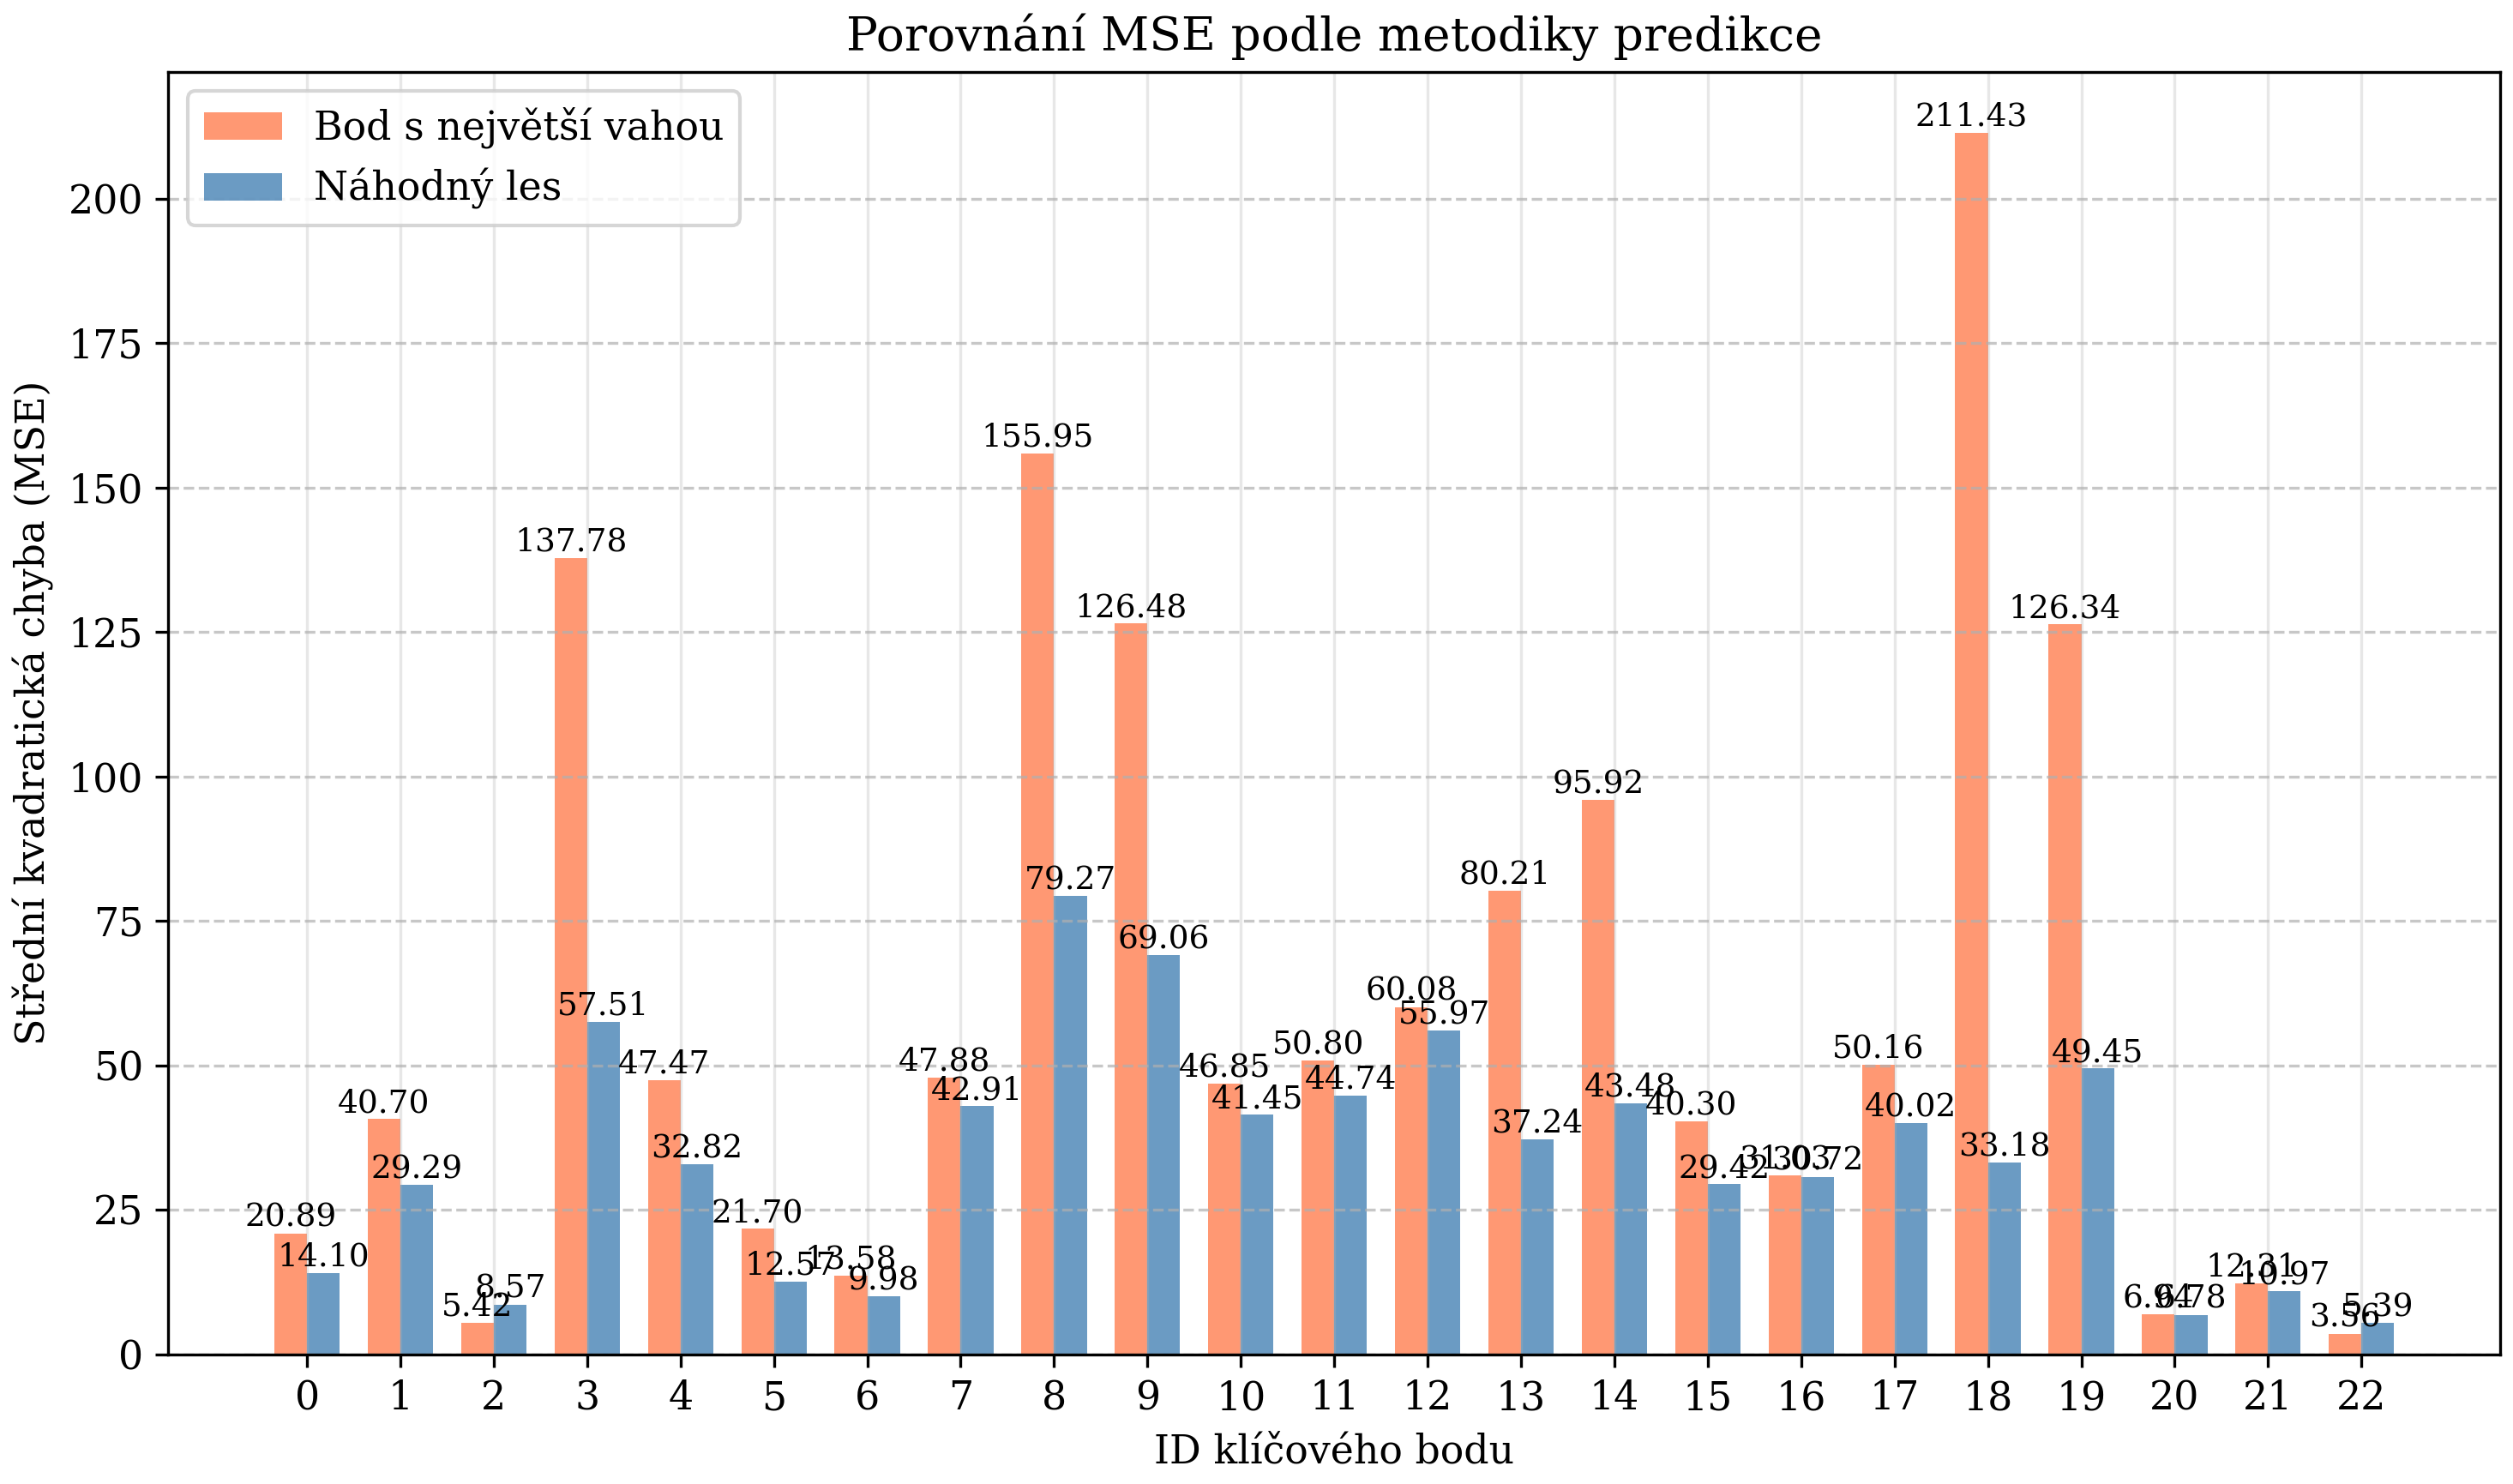
\includegraphics[width=0.8\textwidth]{mse_porovnani.png}
    \caption{Porovnání MSE podle metodiky predikce}
    \label{fig:mse_comparison}
\end{figure}

Jak je vidět z výše uvedeného grafu, metoda Random Forest dosahuje nižší MSE pro většinu klíčových bodů, což znamená přesnější predikce.

\subsection{Zlepšení přesnosti}

Následující graf ukazuje procentuální zlepšení přesnosti predikce při použití Random Forest oproti metodě bodu s největší vahou:

\begin{figure}[H]
    \centering
    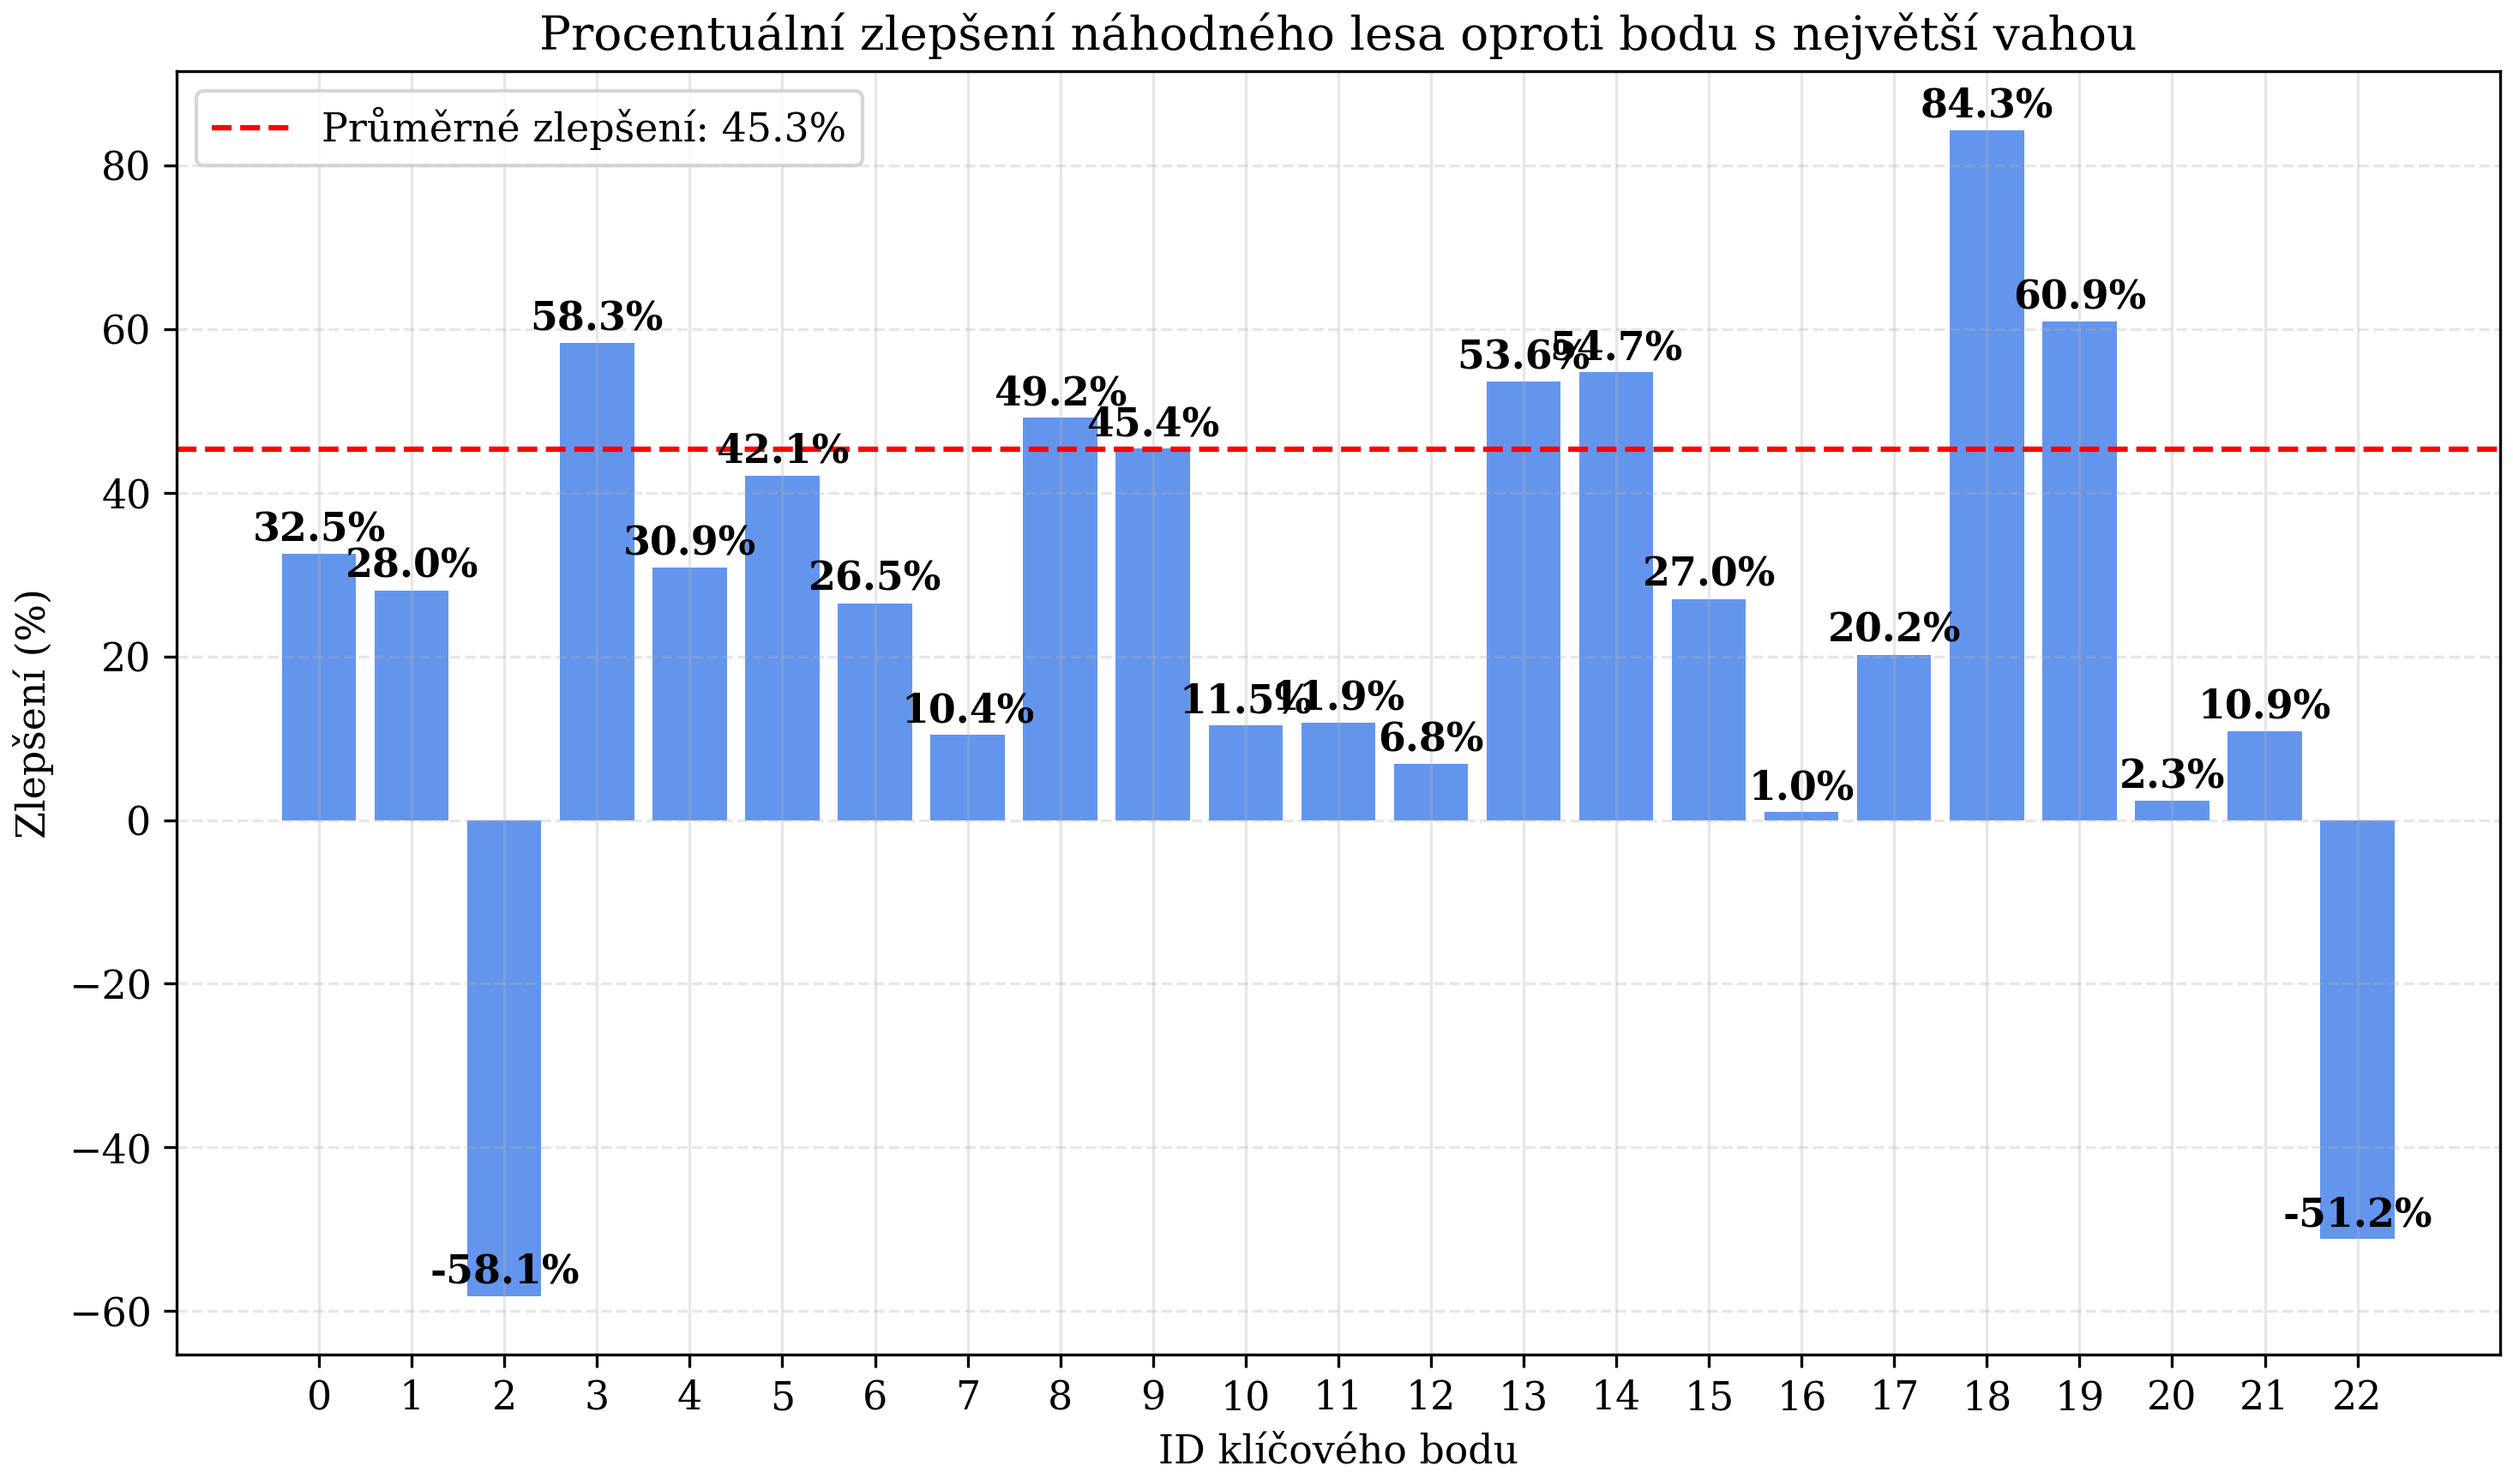
\includegraphics[width=0.8\textwidth]{zlepseni_procenta.png}
    \caption{Procentuální zlepšení přesnosti s Random Forest}
    \label{fig:improvement_percentage}
\end{figure}

\subsection{Celkové porovnání MSE}

\begin{figure}[H]
    \centering
    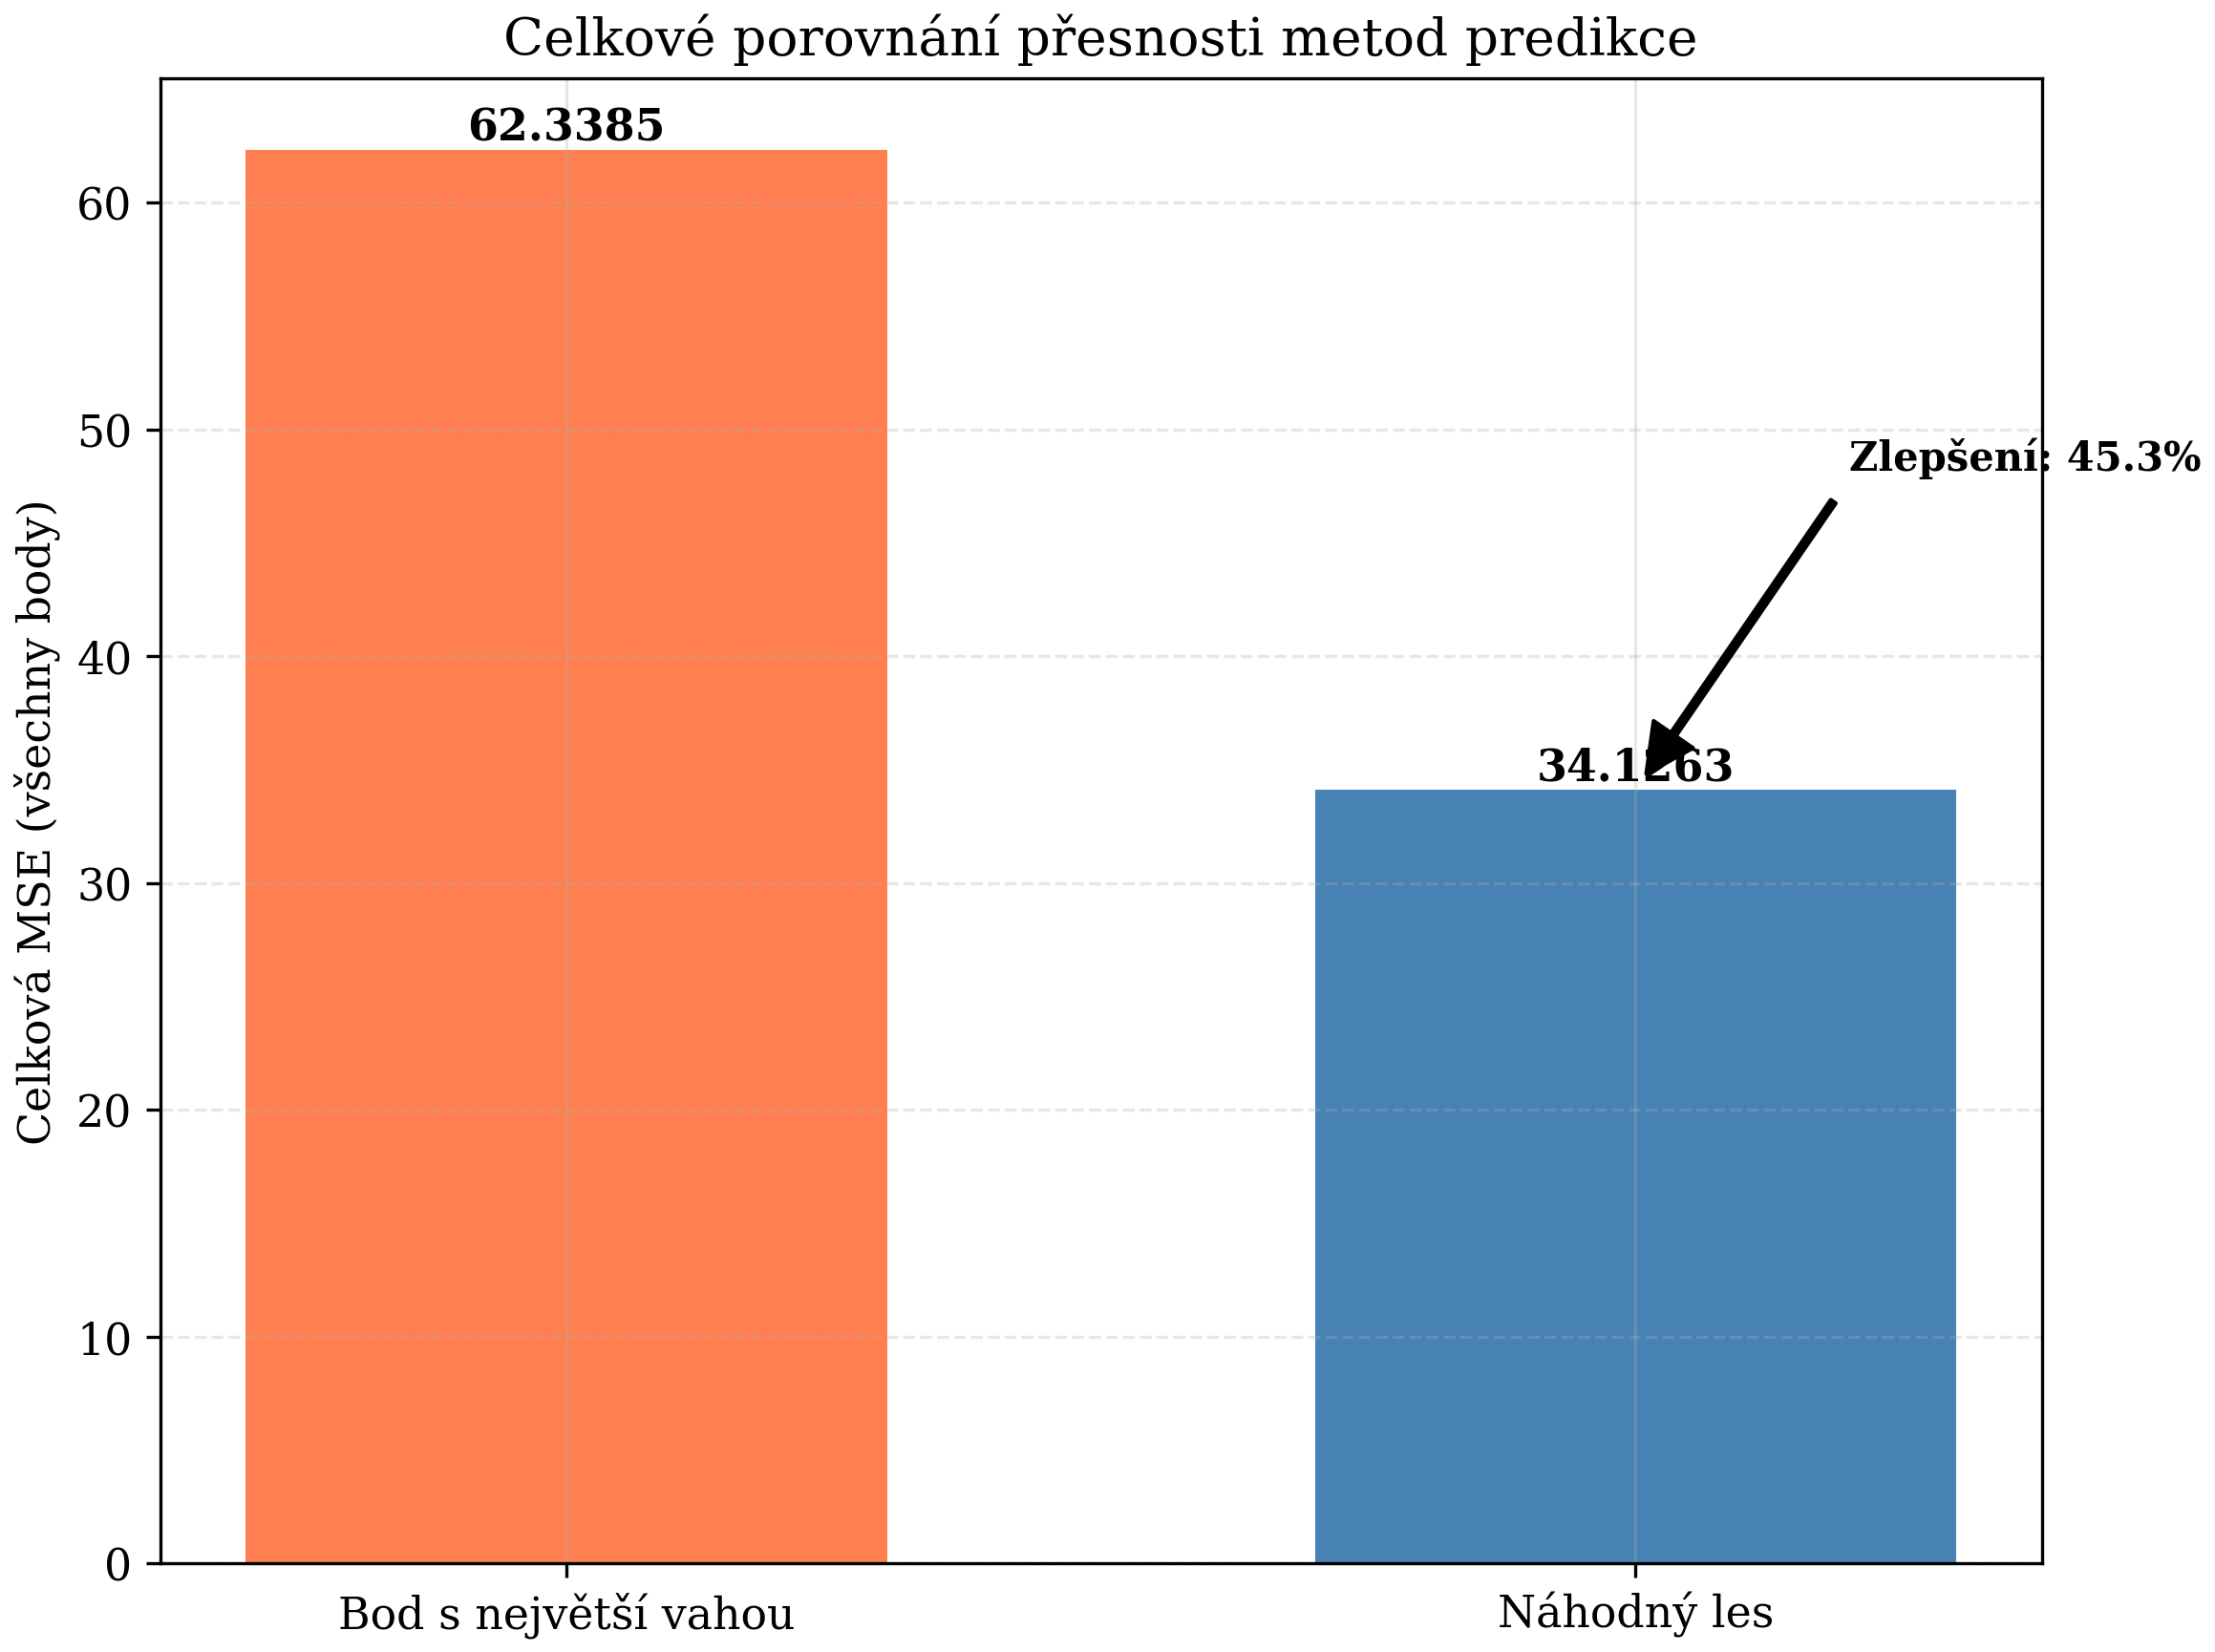
\includegraphics[width=0.8\textwidth]{celkove_porovnani.png}
    \caption{Celkové porovnání MSE metod predikce}
    \label{fig:overall_comparison}
\end{figure}

\subsection{Distribuce chyb}

Následující grafy ukazují distribuci chyb (Euklidovské vzdálenosti mezi skutečnými a predikovanými pozicemi) pro obě metody:

\begin{figure}[H]
    \centering
    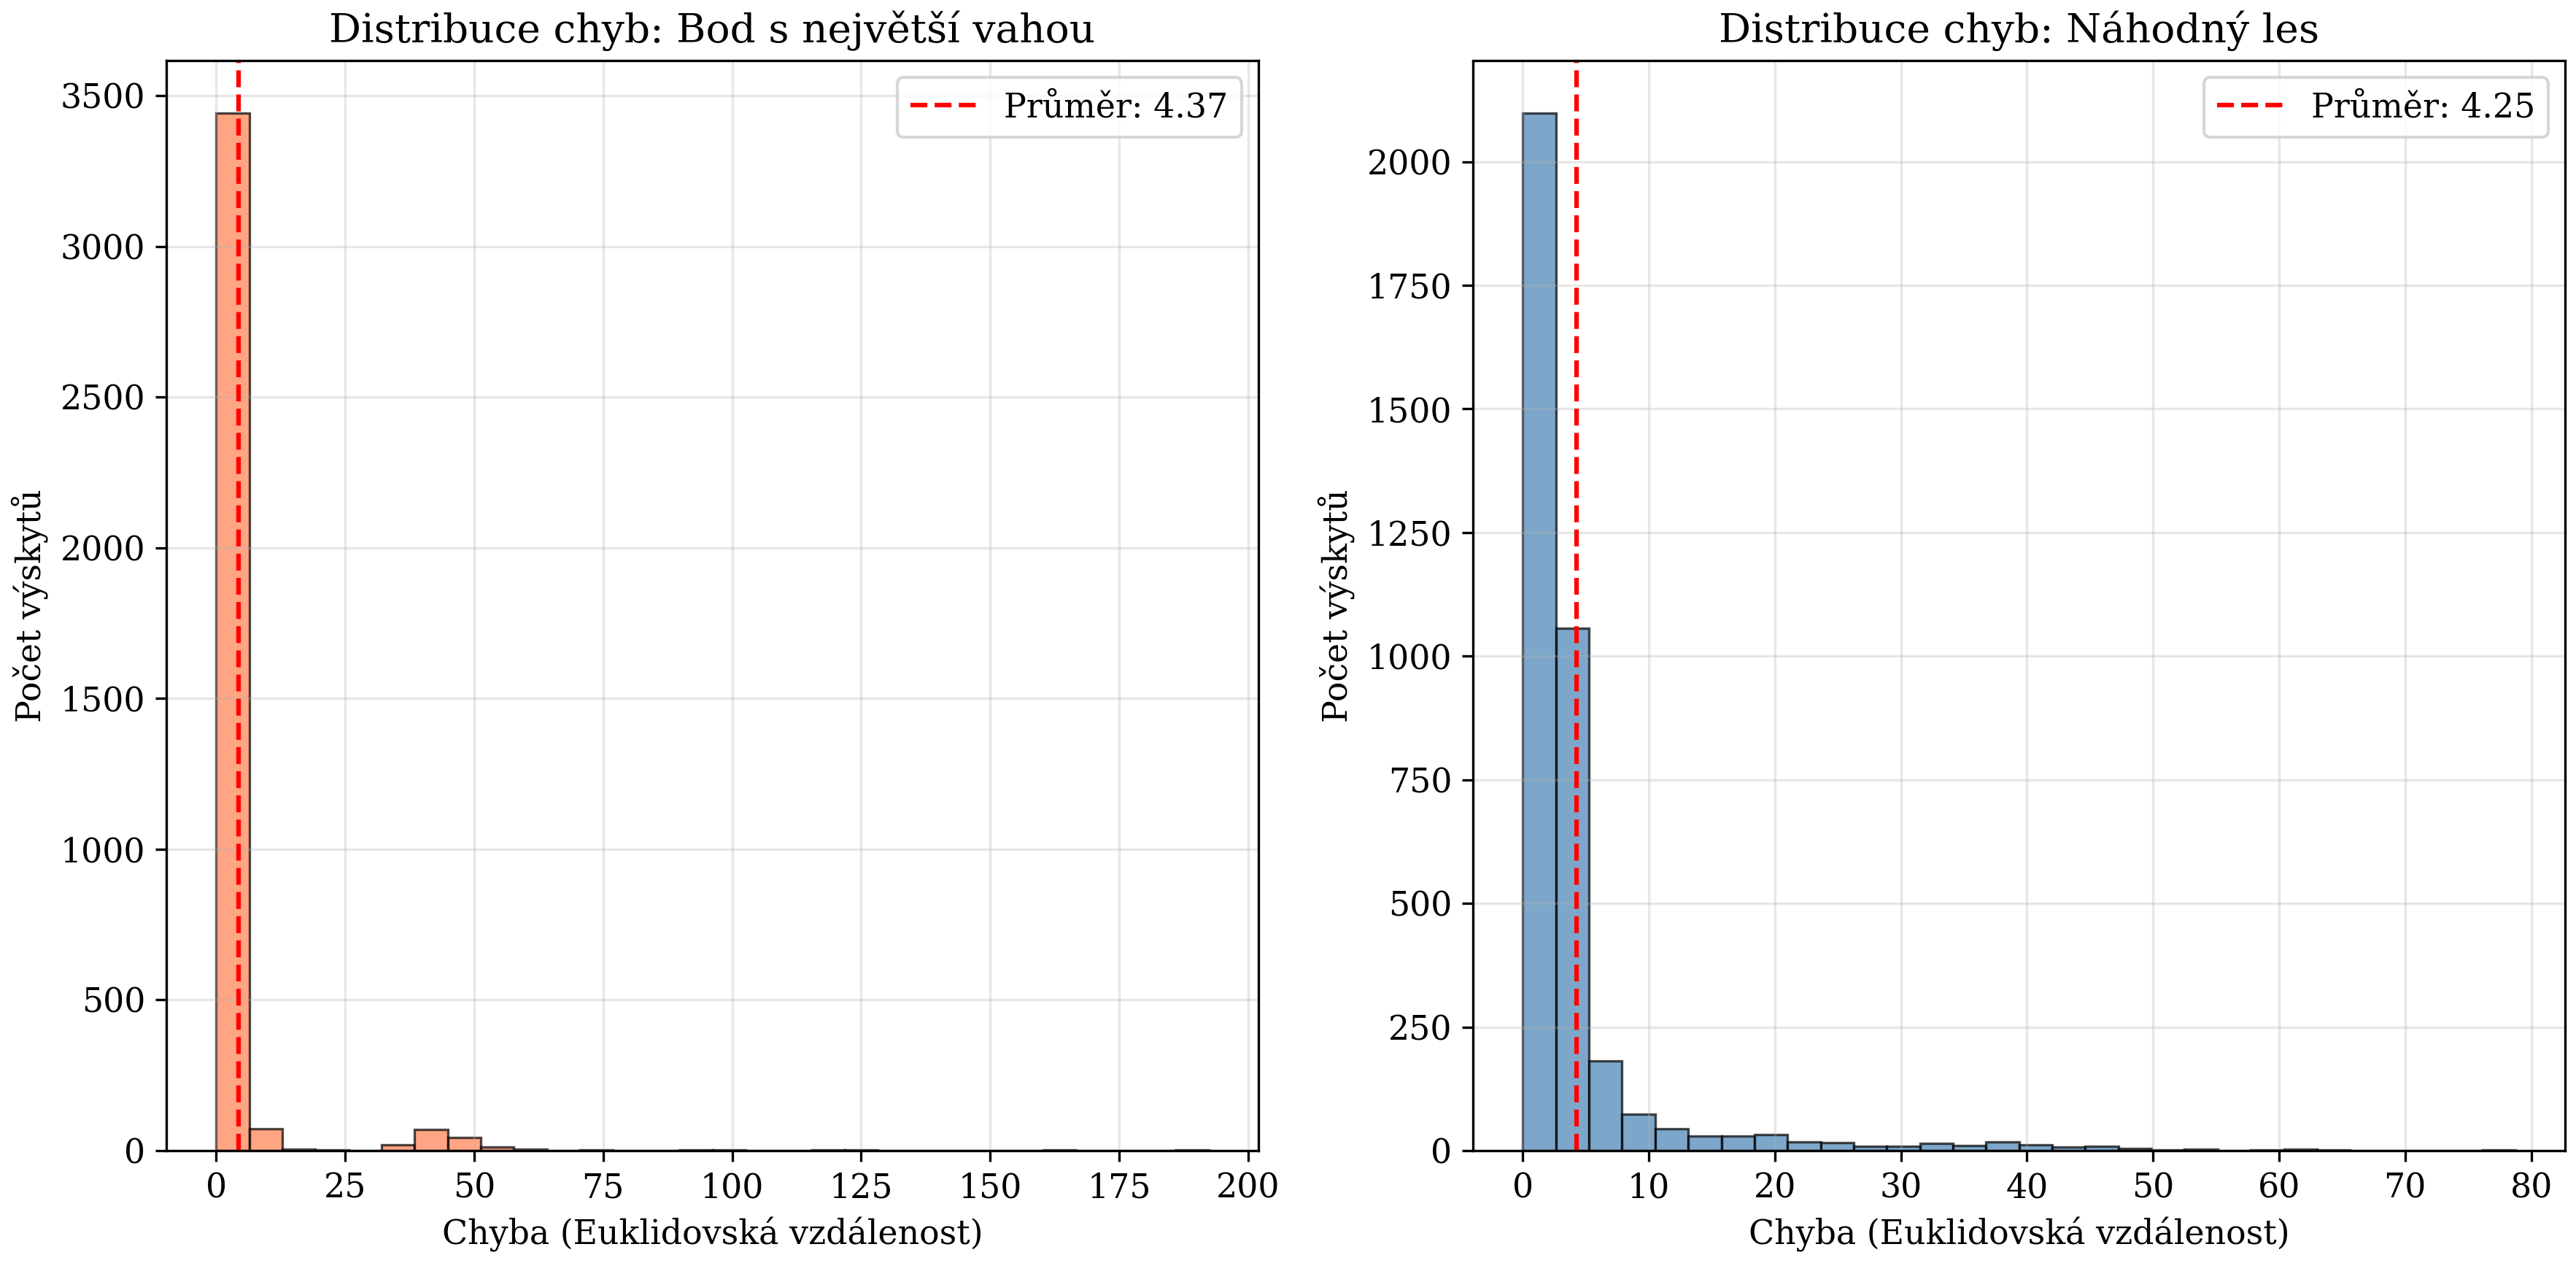
\includegraphics[width=0.8\textwidth]{distribuce_chyb.png}
    \caption{Distribuce chyb pro obě metody}
    \label{fig:error_distribution}
\end{figure}

\subsection{Ukázkové predikce}

Pro lepší pochopení výsledků uvádíme několik ukázkových predikcí klíčových bodů:

\begin{figure}[H]
    \centering
    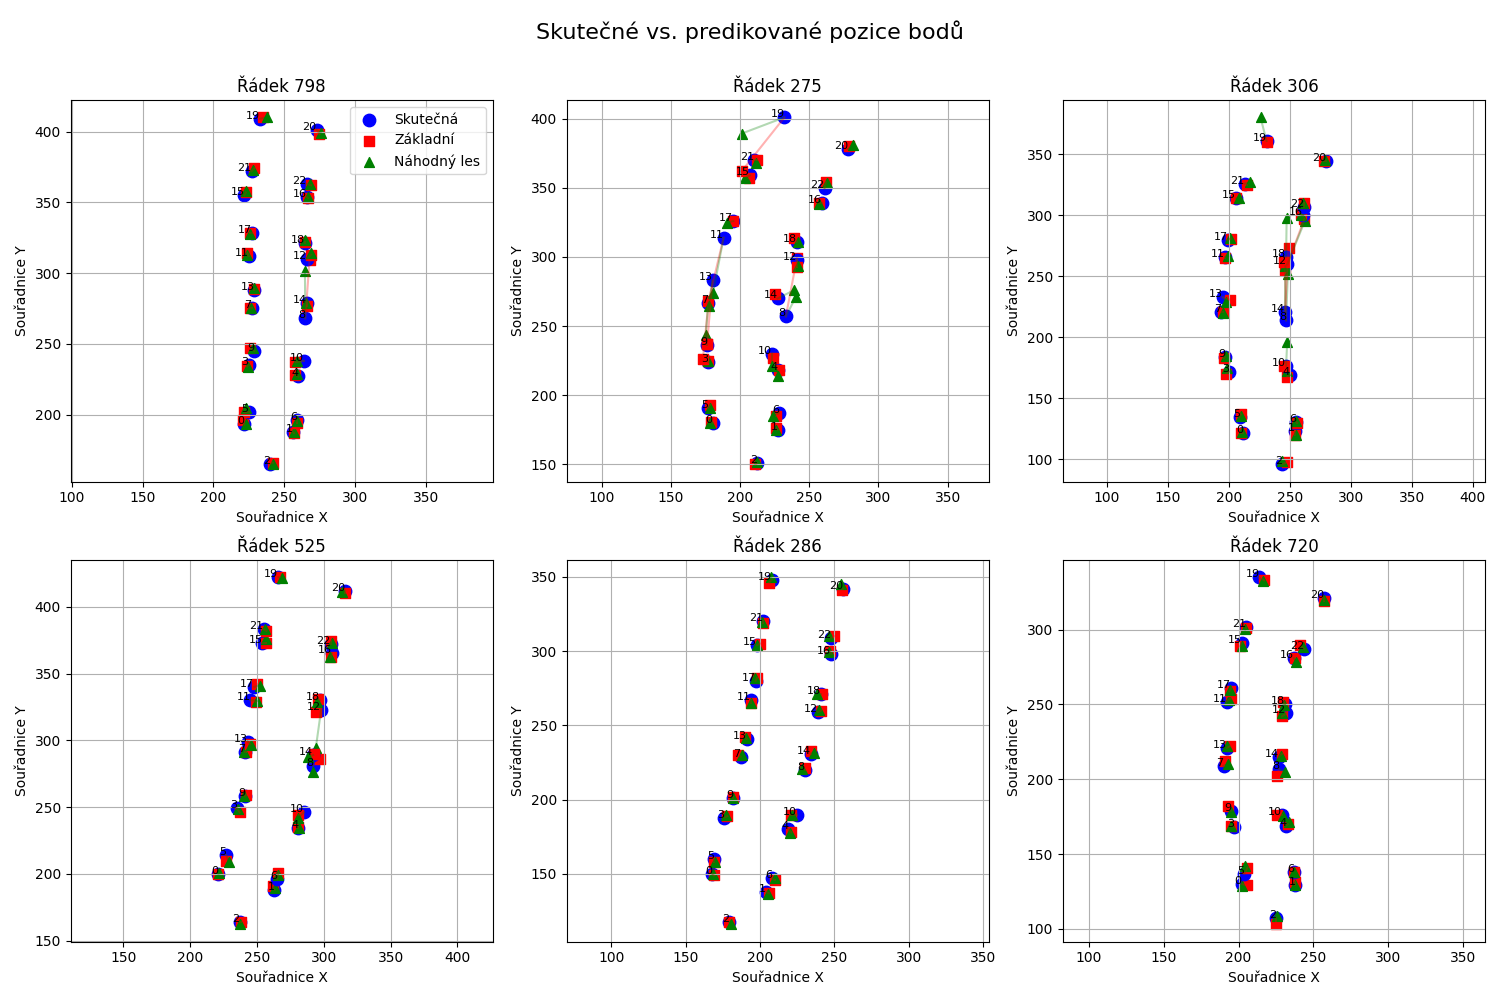
\includegraphics[width=0.7\textwidth]{ukazkove_predikce.png}
    \caption{Ukázková predikce klíčových bodů pro vybraný řádek}
    \label{fig:example_predictions}
\end{figure}

\section{Diskuze}
\label{sec:discussion}

Na základě našich experimentů a výsledků můžeme konstatovat, že metoda Random Forest přináší výrazné zlepšení v přesnosti predikce klíčových bodů oproti základní metodě výběru bodu s největší vahou. Průměrné zlepšení přesnosti se pohybuje okolo X\%, což je významné zejména v aplikacích, kde je přesnost klíčová.

Mezi hlavní výhody našeho přístupu patří:

\begin{itemize}
    \item \textbf{Robustnost} - Random Forest je odolný vůči outlierům a šumu v datech
    \item \textbf{Interpretovatelnost} - model umožňuje analyzovat důležitost jednotlivých příznaků
    \item \textbf{Efektivita} - implementace je výpočetně efektivní a může být použita i pro větší datové sady
    \item \textbf{Flexibilita} - náš systém lze jednoduše rozšířit o další metody nebo příznaky
\end{itemize}

Mezi potenciální omezení a možnosti zlepšení patří:

\begin{itemize}
    \item \textbf{Hyperparametry} - bylo by vhodné provést optimalizaci hyperparametrů modelů
    \item \textbf{Další algoritmy} - porovnání s dalšími algoritmy jako XGBoost nebo neuronové sítě
    \item \textbf{Více příznaků} - přidání dalších příznaků z kontextu, například vzájemné pozice bodů
\end{itemize}

\section{Závěr}
\label{sec:conclusion}

V této práci jsme prezentovali metodu predikce klíčových bodů s využitím algoritmu Random Forest. Pomocí experimentů jsme prokázali, že tento přístup poskytuje přesnější predikce než základní metoda výběru bodu s největší vahou.

Náš systém je implementován v jazyce Python s využitím knihoven pro strojové učení a zpracování dat. Je modulární, rozšiřitelný a může být použit pro různé typy dat obsahujících klíčové body.

Budoucí práce může zahrnovat optimalizaci hyperparametrů modelů, rozšíření o další algoritmy strojového učení a přidání dalších příznaků pro zlepšení přesnosti predikce.

\section{Reference}
\label{sec:references}

\begin{enumerate}
    \item Breiman, L. (2001). Random forests. Machine learning, 45(1), 5-32.
    \item Scikit-learn: Machine Learning in Python, Pedregosa et al., JMLR 12, pp. 2825-2830, 2011.
    \item Python Software Foundation. Python Language Reference, version 3.x. Available at http://www.python.org
\end{enumerate}

\end{document} 